%%%%%%%%%%%%%%%%%%%%%%%%%%%%%%%%%%%%%%%%%%%%%%%%%%%%%%%%%%%%%%%%%%%%%%
% writeLaTeX Example: Academic Paper Template
%
% Source: http://www.writelatex.com
% 
% Feel free to distribute this example, but please keep the referral
% to writelatex.com
% 
%%%%%%%%%%%%%%%%%%%%%%%%%%%%%%%%%%%%%%%%%%%%%%%%%%%%%%%%%%%%%%%%%%%%%%
% How to use writeLaTeX: 
%
% You edit the source code here on the left, and the preview on the
% right shows you the result within a few seconds.
%
% Bookmark this page and share the URL with your co-authors. They can
% edit at the same time!
%
% You can upload figures, bibliographies, custom classes and
% styles using the files menu.
%
% If you're new to LaTeX, the wikibook is a great place to start:
% http://en.wikibooks.org/wiki/LaTeX
%
%%%%%%%%%%%%%%%%%%%%%%%%%%%%%%%%%%%%%%%%%%%%%%%%%%%%%%%%%%%%%%%%%%%%%%
\documentclass[twocolumn,showpacs,%
  nofootinbib,aps,superscriptaddress,%
  eqsecnum,prd,notitlepage,showkeys,10pt]{revtex4-1}

\usepackage[portuguese]{babel}
\usepackage[shortlabels]{enumitem}
\usepackage[utf8]{inputenc}
\usepackage{amssymb}
\usepackage{amsmath}
\usepackage{graphicx}
\usepackage{dcolumn}
\usepackage{xcolor}
\usepackage[pdfstartview=FitH,
            colorlinks,
            bookmarksnumbered,
            bookmarksopen,
            linktocpage,
            urlcolor=blue,
            linkcolor=red!70!black,
            citecolor=red!70!black]{hyperref}
\usepackage{subcaption}
\usepackage{float}
\usepackage{listings}
\usepackage{color}
\usepackage{tikz}
\usetikzlibrary{shapes, arrows}

\tikzstyle{terminator} = [rectangle, draw, text centered, rounded corners, minimum height=2em]
\tikzstyle{process} = [rectangle, draw, text centered, minimum height=2em]
\tikzstyle{decision} = [diamond, draw, text centered, minimum height=2em]
\tikzstyle{data}=[trapezium, draw, text centered, trapezium left angle=60, trapezium right angle=120, minimum height=2em]
\tikzstyle{connector} = [draw, -latex']

\definecolor{dkgreen}{rgb}{0,0.6,0}
\definecolor{gray}{rgb}{0.5,0.5,0.5}
\definecolor{mauve}{rgb}{0.58,0,0.82}

\lstset{frame=tb,
  language=[90]Fortran,
  aboveskip=3mm,
  belowskip=3mm,
  showstringspaces=false,
  columns=flexible,
  basicstyle={\small\ttfamily},
  numbers=none,
  numberstyle=\tiny\color{gray},
  keywordstyle=\color{blue},
  commentstyle=\color{dkgreen},
  stringstyle=\color{mauve},
  breaklines=true,
  breakatwhitespace=true,
  tabsize=4
}

\usepackage[nottoc,numbib]{tocbibind}
\usepackage{physics}

\usepackage[cmintegrals,cmbraces]{newtxmath}
\usepackage{ebgaramond-maths}

\newcommand{\C}{\mathbb{C}}
\newcommand{\R}{\mathbb{R}}
\newcommand{\N}{\mathbb{N}}
\newcommand{\Z}{\mathbb{Z}}

\DeclareMathOperator\erfc{erfc}
\newcommand*\diff{\mathop{}\!\mathrm{d}}
\newcommand*\Diff[1]{\mathop{}\!\mathrm{d^#1}}
\renewcommand{\leq}{\leqslant}
\renewcommand{\geq}{\geqslant}
\newcommand* \e{\mathrm{e}}

\makeatletter
  \DeclareSymbolFont{ntxletters}{OML}{ntxmi}{m}{it}
  \SetSymbolFont{ntxletters}{bold}{OML}{ntxmi}{b}{it}
  \re@DeclareMathSymbol{\leftharpoonup}{\mathrel}{ntxletters}{"28}
  \re@DeclareMathSymbol{\leftharpoondown}{\mathrel}{ntxletters}{"29}
  \re@DeclareMathSymbol{\rightharpoonup}{\mathrel}{ntxletters}{"2A}
  \re@DeclareMathSymbol{\rightharpoondown}{\mathrel}{ntxletters}{"2B}
  \re@DeclareMathSymbol{\triangleleft}{\mathbin}{ntxletters}{"2F}
  \re@DeclareMathSymbol{\triangleright}{\mathbin}{ntxletters}{"2E}
  \re@DeclareMathSymbol{\partial}{\mathord}{ntxletters}{"40}
  \re@DeclareMathSymbol{\flat}{\mathord}{ntxletters}{"5B}
  \re@DeclareMathSymbol{\natural}{\mathord}{ntxletters}{"5C}
  \re@DeclareMathSymbol{\star}{\mathbin}{ntxletters}{"3F}
  \re@DeclareMathSymbol{\smile}{\mathrel}{ntxletters}{"5E}
  \re@DeclareMathSymbol{\frown}{\mathrel}{ntxletters}{"5F}
  \re@DeclareMathSymbol{\sharp}{\mathord}{ntxletters}{"5D}
  \re@DeclareMathAccent{\vec}{\mathord}{ntxletters}{"7E}
\makeatother

\DeclareMathAlphabet\mathbfcal{OMS}{cmsy}{b}{n}

\begin{document}

\title{
Problemas de Sturm-Liouville unidimensionais: 
uma abordagem numérica usando o método do tiro
}
\author{Caio Tomás de Paula}
\affiliation{Departamento de Matemática, Universidade de Brasília, Brasil.}
%
\begin{abstract}
    Relatório entregue como parte da avaliação do curso de Introdução a
    Métodos Computacionais em Equações Diferenciais Ordinárias (IMCEDO),
    ministrado pelo prof. Dr. Yuri Dumaresq Sobral no segundo semestre letivo
    de 2022 da Universidade de Brasília. Foi utilizada 
    \cite{Sturm-Liouville} como referência principal para o trabalho, além
    das notas de aula \cite{notas-aula-IMCEDO}.
\end{abstract}
%
\maketitle
%
\section{Introdução}
%
Em uma dimensão, o problema tem a forma geral
%
\begin{equation}
\label{eq:forma-geral-SL-1D}
    \left\{
    \begin{array}{l}
        -(p(x)y')' + q(x)y = \lambda r(x)y, \, a \leq x \leq b \\
        \alpha y(a) + \beta y'(a) = 0, \\
        \gamma y(b) + \delta y'(b) = 0.
    \end{array}
    \right.
\end{equation}
%
O valor de $\lambda$ não é especificado na equação: encontrar $\lambda$
tal que o problema admita solução não-trivial é parte do problema de Sturm-Liouville.
Tais valores de $\lambda$, quando existem, são chamados \textbf{autovalores}
do problema, e as soluções correspondentes são as autofunções associadas
a cada $\lambda$. Esta terminologia vem do fato de que as soluções correspondem
aos autovalores/autofunções de um operador diferencial definido num espaço
de funções com um produto interno apropriado. 

A teoria de Sturm-Liouville é muito importante, em particular, no contexto
da Matemática Aplicada: problemas de Sturm-Liouville aparecem com muita
frequência, em particular quando se lida com EDPs lineares separáveis.
Alguns exemplos são:
%
\begin{itemize}
    \item a equação do calor;
    \item a equação da onda;
    \item a equação de Poisson;
    \item a equação de Laplace;
    \item a equação de Helmholtz;
    \item a equação de Schrödinger unidimensional independente do tempo.
\end{itemize}
%
Vamos considerar apenas problemas \textbf{regulares}, que satisfazem as condições
%
\begin{enumerate}[(i)]
    \item $p, q > 0$ em $[a,b]$;
    \item $p, q, r\in C^1([a,b])$;
    \item $\alpha, \beta, \gamma, \delta \in\R$ com $|\alpha| + |\beta| > 0$
    e $|\gamma| + |\delta| > 0$.
\end{enumerate}
%
Ademais, para implementarmos o método do tiro vamos requerer que
%
\begin{itemize}
    \item[(iv)] $p, q, r\in C^2([a,b])$.
\end{itemize}
%

dar exemplos de problemas regulares e irregulares que aparecem em MMF1

Em várias dimensões, o problema de autovalor assume a forma da
\textbf{equação de Helmholtz}, dada por
%
\begin{equation}
\label{eq:helmholtz}
    \left\{
    \begin{array}{l}
        \laplacian u + \alpha^2u = 0, \, \mathbf{x}\in\Omega \\
        F(u, u_{x_1}, u_{x_2}, \dots, u_{x_n}) = 0, \mathbf{x}\in\partial\Omega.
    \end{array}
    \right.
\end{equation}
%
O principal resultado da teoria de Sturm-Liouville afirma que
%
\begin{enumerate}
    \item os autovalores são reais e podem ser ordenados,
    %
    \[
        \lambda_1 < \lambda_2 < \cdots < \lambda_n < \cdots \to \infty.
    \]
    %
    \item a cada autovalor $\lambda_n$ está associada uma única (a menos
    de multiplicação por escalar) autofunção $y_n$, que tem exatamente 
    $n-1$ zeros em $(a,b)$, chamada \textbf{$n$-ésima solução fundamental}.

    \item as autofunções (normalizadas) formam uma base ortonormal com
    respeito ao produto interno de peso $r$, i.e.,
    %
    \[
        \left\langle y_n, y_m \right\rangle
        = \int_a^b y_n(x)y_m(x)r(x) \diff x
        = \delta_{mn},
    \]
    %
    sendo $\delta_{mn}$ o delta de Kronecker:
    %
    \[
        \delta_{nm} = \left\{
        \begin{array}{l}
            1, \, n = m \\
            0, \, n\neq m.
        \end{array}
        \right.
    \]
    %
\end{enumerate}
%
Para resolver este problema numericamente, vamos usar o
\textbf{método do tiro}.
%
\section{Resultados}
\label{sec:resultados}
%
\subsection{O método numérico}
%
A ideia do método do tiro é transformar a solução de um PVC na solução
de (alguns) PVIs combinada à solução de uma equação (ou sistema) algébrico,
dada pela solução do PVI.
Para ilustrar o funcionamento do método aplicado a este problema, considere
o problema de autovalor unidimensional com c.c.'s de Dirichlet:
%
\[
    \left\{
    \begin{array}{l}
        y'' + \lambda y = 0, \, a \leq x \leq b \\
        y(a) = 0 = y(b).
    \end{array}
    \right.
\]
%
Se $\lambda$ é um autovalor e $y(x) = y(x,\lambda)$ é a autofunção correspondente,
então $y'(a) \neq 0$ e, portanto, existe uma única autofunção normalizada com $y'(a) = 1$.
Esta autofunção normalizada deve satisfazer o PVI
%
\[
    \left\{
    \begin{array}{l}
        u'' + \lambda u = 0, \, a \leq x \leq b \\
        u(a) = 0, \, u'(a) = 1
    \end{array}
    \right.
\]
%
e, também, a equação $u(b) = u(,b\lambda) = 0$. Reciprocamente, se $u$ é solução
do PVI anterior e é tal que $u(b,\lambda) = 0$, então $\lambda$ é um autovalor
do problema de Sturm-Liouville e $y(x) = u(x,\lambda)$ é a autofunção normalizada correspondente.

De maneira geral, se temos o problema \eqref{eq:forma-geral-SL-1D}, então o PVI associado é
%
\begin{equation}
\label{eq:PVI-geral-tiro}
    \left\{
        \begin{array}{l}
            -(p(x)u')' + (q(x) - \lambda r(x))u = 0, \, a \leq x \leq b \\
            u(a) = -\beta/\sqrt{\alpha^2 + \beta^2}, \,
            u'(a) = \alpha/\sqrt{\alpha^2 + \beta^2}.
        \end{array}
    \right.
\end{equation}
%
Pela simplicidade dos autovalores e unicidade das autofunções,
segue que a única autofunção (normalizada) associada a cada autovalor é tal que
%
\[
    y(a) = -\beta/\sqrt{\alpha^2 + \beta^2}, \,
    y'(a) = \alpha/\sqrt{\alpha^2 + \beta^2}.
\]
%
Assim, resolver o  PVC \eqref{eq:forma-geral-SL-1D} é equivalente a resolver o PVI \eqref{eq:PVI-geral-tiro}
e encontrar a raiz de $F(\lambda) = 0$, sendo
%
\begin{equation}
\label{eq:eq-algebrica-tiro}
    F(\lambda) = \gamma u(b, \lambda) + \delta u'(b, \lambda).
\end{equation}
%
Feito isto, a autofunção normalizada é $y(x) = u(x,\lambda)$.

Portanto, resolver o PVC é \textbf{equivalente} (tanto conceitual quanto numericamente)
a resolver o PVI e a equação $u(b,\lambda) = 0$.

Essencialmente, o algoritmo é:
%
\begin{enumerate}
    \item propor uma estimativa $\lambda_n^i$ para o autovalor $\lambda_n$; 
    \item resolver o PVI em $u(x, \lambda_n^i)$ dado por \eqref{eq:PVI-geral-tiro};
    \item avaliar o quão longe de $0$ está $F(\lambda)$:
    %
    \begin{enumerate}
        \item se muito longe, usamos um método iterativo para obter um próximo 
        chute $\lambda_n^{i+1}$ e voltamos ao passo 1;
        \item se perto o bastante, paramos: o autovalor foi encontrado;
        \item encontrado o autovalor, resolvemos o PVI \eqref{eq:PVI-geral-tiro} uma
        última vez para determinar a autofunção associada.
    \end{enumerate}
    %
\end{enumerate}
%
É possível mostrar (cf. \cite[p.~304-305, Teo.~186 - 188]{Sturm-Liouville}) que
podemos usar os métodos da bisseção e de Newton-Raphson para encontrar os autovalores
em problemas de Sturm-Liouville regulares\footnote{Os mesmos resultados valem, com as devidas
alterações nas demonstrações, para problemas de Sturm-Liouville singulares.}.

\begin{figure}[H]
    \centering
    \begin{tikzpicture}[node distance = 2cm]
        \node [terminator, fill=blue!20] (start) {\textbf{Inicialização variáveis}};
        % \node [process, fill=blue!20] at (0,-1.5) (PVI1) 
        % {Resolver o PVI \eqref{eq:PVI-geral-tiro} para $\lambda = a$};
        \node [process, fill=blue!20] at (0,-1.5) (PVI2) 
        {Resolver o PVI \eqref{eq:PVI-geral-tiro} para $\lambda = \lambda_n^i$};
        \node [decision, fill=blue!20, below of = PVI2] (decision) {$F(\lambda_n^i) < \mathrm{TOL}$?};
        \node [process, fill=red!20] at (3.7,-1.5) (chute) 
        {$\lambda_n^i \to \lambda_n^{i+1}$};
        \node [process, fill=green!20] at (0,-6) (encontrado)
        {Autovalor $\lambda_n^*$ encontrado!};
        \node [process, fill=blue!20] at (0,-7.5) (PVIFinal) 
        {Resolver o PVI \eqref{eq:PVI-geral-tiro} para $\lambda = \lambda_n^*$};
        \node [data, fill=blue!20] at (0,-9) (salvamento) 
        {Salvar solução};
        \node [terminator, fill=blue!20] at (0,-10.5) (end) {\textbf{Fim}};
        
        \node[draw=none] at (2.00, -2.72) (no) {Não};
        \node[draw=none] at (0.35, -5.20) (yes) {Sim};
        
        \path [connector] (start) -- (PVI2);
        \path [connector] (PVI2) -- (decision);
        \path [connector] (decision) -- (chute);
        \path [connector] (decision) -- (encontrado);
        \path [connector] (chute) -- (PVI2);
        \path [connector] (encontrado) -- (PVIFinal);
        \path [connector] (PVIFinal) -- (salvamento);
        \path [connector] (salvamento) -- (end);
    \end{tikzpicture}
    \caption{Fluxograma do código}
    \label{fig:flux-codigo}
\end{figure}
%
\subsection{Validação do método}\label{subsec:validacao}
%
Para testar e validar o método, resolvemos o problema de Sturm-Liouville
%
\[
    \left\{
        \begin{array}{l}
            y'' + \lambda y = 0, \, 0 \leq x \leq 1 \\
            y(0) = y(1) = 0,
        \end{array}
    \right.
\]
%
cujos autovalores e autofunções podem ser calculados sem dificuldades e são dados por
%
\[
    \lambda_n = n^2\pi^2, \, y_n = \sin(n\pi x).
\]
%
Resolvendo este PVC com chutes iniciais para a bisseção $[a,b] = [n^2\pi^2 -2, n^2\pi^2 + 5]$, 
encontramos as autofunções da Figura \ref{fig:first-problem}.
Traçamos as autofunções normalizadas na Figura \ref{fig:first-problem-check}, mostrando
que o método encontrou corretamente os autovalores e as autofunções.
%
\begin{figure*}
    \centering
    \begin{minipage}[b]{.49\textwidth}
        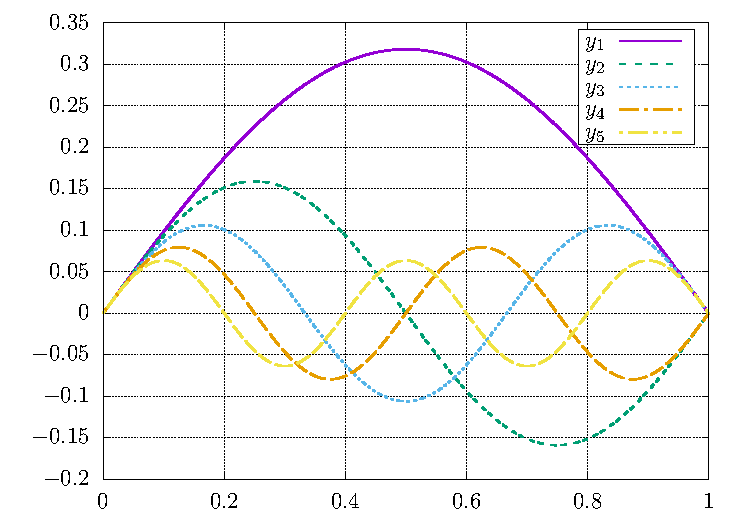
\includegraphics[width=\textwidth]{Relatório/Figuras/FirstProblem.pdf}
        \caption{Gráficos das primeiras cinco autofunções normalizadas
        encontradas numericamente.}\label{fig:first-problem}
    \end{minipage}\hfill
    \begin{minipage}[b]{.49\textwidth}
        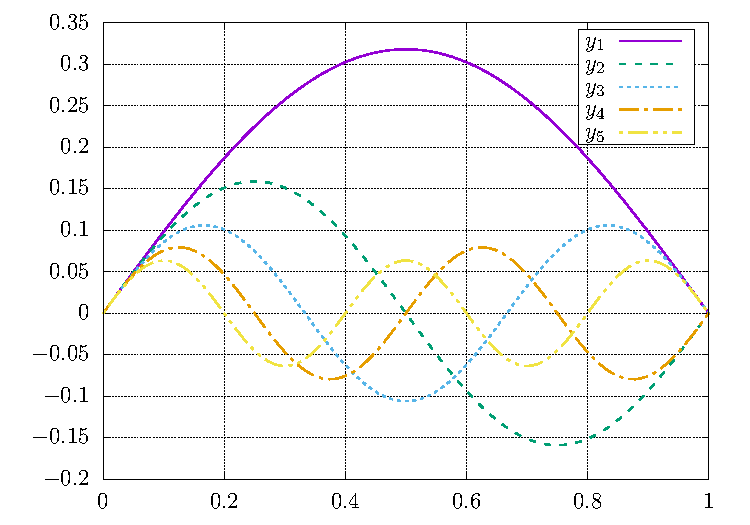
\includegraphics[width=\textwidth]{Relatório/Figuras/FirstProblem_check.pdf}
        \caption{Gráficos das primeiras 5 autofunções normalizadas, $\sin(n\pi x)/(n\pi)$.}\label{fig:first-problem-check}
    \end{minipage}
\end{figure*}
%

%
\subsection{Aplicando o método}\label{subsec:aplicacao}
%

asdasd

%
\subsection{Conclusão}\label{subsec:conclusao}
%

asdasd

% \lstinputlisting[language=Fortran, caption=Teste]{Codes/teste_programa.f90}

% \begin{acknowledgments}

% We thank\dots

% \end{acknowledgments}

% \newpage
% \nocite{*}
% \bibliographystyle{apalike}
\bibliographystyle{siam}
\bibliography{referencias}

\end{document}